\subsection{Descrizione del task}
Il \textbf{Named Entity Recognition (NER)} è uno dei compiti di pre-elaborazione dei dati. Comporta l'identificazione delle entità chiave nel testo e la classificazione di esse in un insieme di categorie predefinite. Un'entità è fondamentalmente la cosa di cui si parla o a cui ci si riferisce costantemente nel testo.

Per imparare cos'è un'entità, un modello NER deve essere in grado di rilevare una parola, o una stringa di parole che formano un'entità (ad esempio \textit{New York City}), e sapere a quale categoria appartiene. Esistono diversi modi di approcciarsi a questo task:
\begin{itemize}
    \item Un metodo è quello di addestrare il modello per la \textbf{classificazione multi classe} utilizzando diversi algoritmi di Machine Learning, ma è un compito molto impegnativo. Innanzitutto esso richiede un sacco di etichettatura ed inoltre il modello richiede anche una profonda comprensione del contesto per affrontare l'ambiguità delle frasi. 
    \item Un altro modo è il \textbf{Conditional Random Field}\textsuperscript{\cite{ravishchawla_crf}}. È un modello probabilistico che può essere usato per modellare dati sequenziali come le parole. Il CRF può catturare una profonda comprensione del contesto della frase.
    \item il \textbf{Deep Learning Based NER} è molto più accurato del metodo precedente, poiché è in grado di assemblare le parole. Questo è dovuto al fatto che usa il word embedding, che è in grado di capire la relazione semantica e sintattica tra le varie parole. È anche in grado di apprendere l'analisi di parole specifiche per l'argomento e di alto livello automaticamente. Questo rende il deep learning NER applicabile per eseguire più compiti. 
    
    La tecnologia utilizzata in questo progetto per risolvere il task di Named Entity Recognition è basata proprio sul Deep Learning e sfrutta embedding generati dal testo grazie all'utilizzo di modelli preaddestrati presenti in Spark NLP. 
\end{itemize}

Il Named Entity Recognition viene usato per elaborare grandi quantità di contenuti testuali. Un algoritmo per l’estrazione delle entità può trovare persone, organizzazioni, prodotti, luoghi e diverse altre entità all’interno di interi libri, documenti e articoli vari. Queste informazioni possono poi essere utilizzare per la \textbf{categorizzazione automatica} sulla base della quale i risultati di ricerca possono essere compilati in modo più preciso, i contenuti possono essere curati in \textbf{cluster tematici}, i post relativi ai contenuti possono essere mostrati all'utente o la \textbf{pubblicità mirata} può essere riprodotta. Oltre ad essere utilizzate nei portali di notizie, le caratteristiche di raccomandazione dei servizi di media si basano anche sul riconoscimento delle entità nominate. Un altro campo di applicazione oltre all'industria dei media sarebbe il servizio di \textbf{Google AdSense} o l'ordinamento delle richieste di supporto via e-mail o chat.

Non ci sono \textbf{standard di etichettatura}. Le etichette sono in gran parte orientate secondo la necessità dell'applicazione: generalmente si usano le classi di etichette radice \textit{Persona}, \textit{Organizzazione}, \textit{Prodotto}, \textit{Luoghi}, alle quali si aggiungono le etichette di durata e quantità (\textit{tempo} e \textit{quantità}). A queste entità radice viene poi aggiunto un secondo livello gerarchico: \textit{Organizzazione Commerciale}, \textit{Organizzazione Non profit} per esempio, permettono di affinare la descrizione delle entità. 

In campagne recenti (Ester 2\textsuperscript{\cite{Galliano09theester}} e Automatic Content Extraction (ACE)\textsuperscript{\cite{Doddington2004TheAC}}) ci sono 5-6 classi radice, e un totale di 40-50 classi con sottosezioni di etichettatura. Alcuni sistemi di motori di domande e risposte (che usano entità nominate) possono usare diverse centinaia di classi.

Alcuni degli esempi e dei casi d'uso più comuni per il riconoscimento delle entità nominate sono i seguenti:

\begin{itemize}
    \item \textbf{Categorizzazione dei ticket del supporto clienti}: i grandi marchi e le aziende devono esaminare regolarmente una migliaia di ticket di assistenza clienti. L'estrazione di entità nominate può aiutare a categorizzare questi ticket di assistenza clienti in base alla domanda per poi assegnarli al giusto responsabile dell'assistenza clienti. 
    \item \textbf{Raccomandazione di contenuto}: molte applicazioni moderne e siti web di e-commerce si basano su sistemi di raccomandazione per migliorare l'esperienza complessiva dell'utente. Un grande esempio di questo è rappresentato dalle piattaforme di streaming video ampiamente utilizzate come Netflix e YouTube. Usano il named entity recognition per analizzare la cronologia di ricerca degli utenti e raccomandare suggerimenti basati su di essa. 
    \item \textbf{Estrarre informazioni dal feedback dei clienti}: le recensioni online su varie piattaforme sono una grande fonte di feedback. Possono aiutare a identificare cosa piace e cosa no ai clienti. L'estrazione di entità nominate può aiutare a categorizzare le recensioni e ad identificare i problemi ricorrenti.
    \item \textbf{Processamento dei curricula}: trovare un candidato capace non è un compito facile, i reclutatori devono passare manualmente attraverso un sacco di curricula e analizzare le loro qualifiche, abilità, esperienza e altro. Questo può richiedere una notevole quantità di tempo, rendendolo un processo lungo e noioso. L'estrazione di entità nominate viene spessa utilizzata per analizzare il testo in tonnellate di curricula per trovare i candidati più idonei.
    \item \textbf{Annotazione semantica}: l'annotazione semantica può essere definita come il processo di combinare vari pezzi di informazione a concetti come persone, luoghi e cose. A differenza delle annotazioni tipiche, le annotazioni semantiche coinvolgono l'identificazione e l'analisi del testo, l'estrazione di concetti, l'estrazione di relazioni e l'indicizzazione. 
    
    Durante la fase di sperimentazione si è deciso di trattare nello specifico proprio questo compito.
\end{itemize}

\begin{figure}[hbt!]
    \centering
    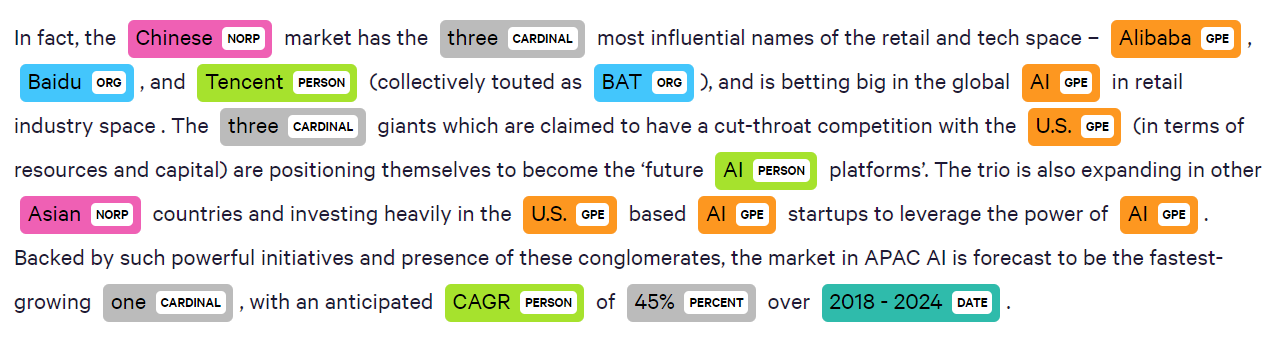
\includegraphics[width=1\textwidth]{img/ner_example.png}
    \caption{NER: annotazione semantica}
    \label{fig:ner_example}
\end{figure}